\chapter{Enhanced Detection Approach}

\section{Motivation for Enhanced Detection}

Traditional clustering algorithms provide a foundation for PUEA detection by separating transmissions into groups based on feature similarity. However, these algorithms have inherent limitations when facing challenging scenarios, particularly when:

\begin{itemize}
    \item The spatial separation between the PU and PUEA is small (as in Scenario C)
    \item Environmental conditions create significant variance in signal propagation
    \item The feature space has regions of overlap between legitimate and malicious transmissions
    \item The clusters have complex structures that deviate from algorithm assumptions
\end{itemize}

The motivation for developing an enhanced detection approach stems from these limitations and the observation that cluster assignments alone may not fully exploit the information contained in the feature space. Traditional clustering provides a macro-level organization of the data, but further refinement within these clusters can potentially improve detection performance.

The enhanced approach introduced in this chapter applies a second-stage detection algorithm (KNN or Means) within established clusters to refine the classification decisions. This two-stage framework leverages the complementary strengths of different algorithms: traditional clustering handles the initial data organization, while the refined methods exploit local patterns within clusters for more accurate detection.

\section{KNN Algorithm within Clusters}

The K-Nearest Neighbors (KNN) algorithm is a non-parametric method used for classification based on proximity in the feature space. In the enhanced detection framework, KNN is applied within each cluster identified by the traditional clustering algorithm to refine the classification decision.

\subsection{Algorithm Description and Pseudocode}

The KNN-enhanced detection algorithm operates on the premise that within a cluster, time slots that are outliers relative to their local neighborhood are potential misclassifications. By examining the k-nearest neighbors of each point within its cluster, the algorithm can identify and potentially reclassify these outliers.

Algorithm \ref{alg:knn_enhanced} presents the pseudocode for KNN-enhanced detection.

\begin{algorithm}
\caption{KNN-Enhanced Detection}
\label{alg:knn_enhanced}
\begin{algorithmic}[1]
\Require Feature vectors $Y_1, Y_2, \ldots, Y_T$, cluster assignments $C$, parameter $k$
\Ensure Refined classification of time slots as PU or PUEA

\State Apply traditional clustering to obtain initial cluster assignments $C$
\State $C_{PU} \gets$ cluster(s) identified as containing PU transmissions
\State $C_{PUEA} \gets$ cluster(s) identified as containing PUEA transmissions

\For{each time slot $t$ in $C_{PU}$}
    \State Find $k$ nearest neighbors of $Y_t$ within $C_{PU}$
    \State Calculate average distance $d_{avg}$ to the $k$ nearest neighbors
    \State Calculate distance $d_{cent}$ to $C_{PU}$ centroid
    \State Calculate distance $d_{other}$ to $C_{PUEA}$ centroid
    \State $r = \frac{d_{avg}}{d_{cent}} \cdot \frac{d_{cent}}{d_{other}}$
    \If{$r > \theta_{PU}$}
        \State Reclassify time slot $t$ as PUEA transmission
    \EndIf
\EndFor

\For{each time slot $t$ in $C_{PUEA}$}
    \State Find $k$ nearest neighbors of $Y_t$ within $C_{PUEA}$
    \State Calculate average distance $d_{avg}$ to the $k$ nearest neighbors
    \State Calculate distance $d_{cent}$ to $C_{PUEA}$ centroid
    \State Calculate distance $d_{other}$ to $C_{PU}$ centroid
    \State $r = \frac{d_{avg}}{d_{cent}} \cdot \frac{d_{cent}}{d_{other}}$
    \If{$r > \theta_{PUEA}$}
        \State Reclassify time slot $t$ as PU transmission
    \EndIf
\EndFor

\end{algorithmic}
\end{algorithm}

\subsection{Parameter Selection ($k=3$)}

The selection of the parameter $k$ (number of neighbors) significantly influences the KNN algorithm's performance. After extensive experimentation with different values, $k=3$ was selected as the optimal value for PUEA detection for several reasons:

\begin{itemize}
    \item \textbf{Local Representation:} $k=3$ provides sufficient local representation without excessive smoothing
    \item \textbf{Computational Efficiency:} Smaller $k$ values reduce computational complexity
    \item \textbf{Robustness to Outliers:} Using 3 neighbors rather than a single neighbor provides robustness against individual anomalous points
    \item \textbf{Empirical Performance:} Experiments across all scenarios showed that $k=3$ consistently provided the best balance between detection rate and false alarm rate
\end{itemize}

Figure \ref{fig:knn_parameter} illustrates the impact of different $k$ values on the detection performance across the three scenarios.

\begin{figure}[htbp]
    \centering
    % This is a placeholder for a figure showing the impact of k parameter
    % In actual thesis, replace this with a real TikZ plot or imported figure
    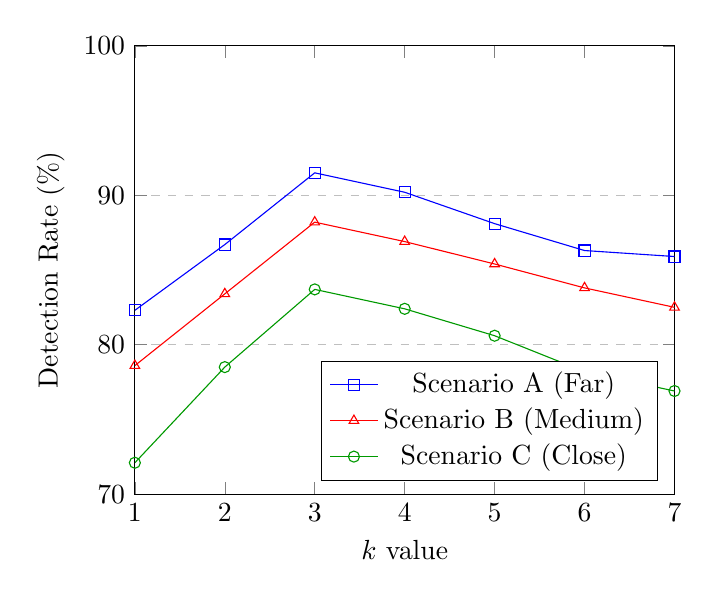
\begin{tikzpicture}
        \begin{axis}[
            xlabel={$k$ value},
            ylabel={Detection Rate (\%)},
            xmin=1, xmax=7,
            ymin=70, ymax=100,
            xtick={1,2,3,4,5,6,7},
            legend pos=south east,
            ymajorgrids=true,
            grid style=dashed,
        ]
        
        \addplot[
            color=blue,
            mark=square,
            ]
            coordinates {
            (1,82.3)(2,86.7)(3,91.5)(4,90.2)(5,88.1)(6,86.3)(7,85.9)
            };
        \addlegendentry{Scenario A (Far)}
            
        \addplot[
            color=red,
            mark=triangle,
            ]
            coordinates {
            (1,78.6)(2,83.4)(3,88.2)(4,86.9)(5,85.4)(6,83.8)(7,82.5)
            };
        \addlegendentry{Scenario B (Medium)}
        
        \addplot[
            color=green!60!black,
            mark=o,
            ]
            coordinates {
            (1,72.1)(2,78.5)(3,83.7)(4,82.4)(5,80.6)(6,78.2)(7,76.9)
            };
        \addlegendentry{Scenario C (Close)}
            
        \end{axis}
    \end{tikzpicture}
    \caption{Effect of $k$ parameter on detection performance across scenarios}
    \label{fig:knn_parameter}
\end{figure}

\subsection{Distance Calculation within Clusters}

The distance between feature vectors within clusters is calculated using the weighted Manhattan distance, consistent with the approach used in traditional clustering:

\begin{equation}
    d_{weighted}(Y_t, Y_{t'}) = \sum_{j=1}^{n} w_j |Y_{t,j}^{\text{norm}} - Y_{t',j}^{\text{norm}}|
\end{equation}

where $w_j$ is the weight assigned to feature $j$ based on its discriminative power as described in Chapter 4.

\subsection{Threshold Determination for Outlier Detection}

A critical aspect of the KNN-enhanced detection is determining appropriate thresholds ($\theta_{PU}$ and $\theta_{PUEA}$) for outlier detection and potential reclassification. These thresholds are determined adaptively based on the distribution of distances within each cluster:

\begin{equation}
    \theta_{PU} = \mu_{PU} + \lambda_{PU} \cdot \sigma_{PU}
\end{equation}

\begin{equation}
    \theta_{PUEA} = \mu_{PUEA} + \lambda_{PUEA} \cdot \sigma_{PUEA}
\end{equation}

where:
\begin{itemize}
    \item $\mu_{PU}$ and $\mu_{PUEA}$ are the mean values of the ratio $r$ for the PU and PUEA clusters, respectively
    \item $\sigma_{PU}$ and $\sigma_{PUEA}$ are the standard deviations of the ratio $r$ for the PU and PUEA clusters, respectively
    \item $\lambda_{PU}$ and $\lambda_{PUEA}$ are scaling factors
\end{itemize}

Based on empirical optimization, the scaling factors were set to:
\begin{itemize}
    \item Scenario A (Far): $\lambda_{PU} = 1.8$, $\lambda_{PUEA} = 2.0$
    \item Scenario B (Medium): $\lambda_{PU} = 1.5$, $\lambda_{PUEA} = 1.7$
    \item Scenario C (Close): $\lambda_{PU} = 1.2$, $\lambda_{PUEA} = 1.5$
\end{itemize}

The decreasing trend in scaling factors across scenarios reflects the need for more sensitive outlier detection in challenging scenarios with closer proximity between PU and PUEA.

\section{Means Algorithm within Clusters}

The Means algorithm represents an alternative enhanced detection approach that relies on the mean distance to all points within a cluster rather than just the k-nearest neighbors. This approach provides a global perspective on outliers within each cluster.

\subsection{Algorithm Description and Pseudocode}

The Means-enhanced detection algorithm identifies outliers by comparing the mean distance from a point to all other points in its cluster against adaptive thresholds. Points with unusually large mean distances are potential misclassifications that may need to be reassigned.

Algorithm \ref{alg:means_enhanced} presents the pseudocode for Means-enhanced detection.

\begin{algorithm}
\caption{Means-Enhanced Detection}
\label{alg:means_enhanced}
\begin{algorithmic}[1]
\Require Feature vectors $Y_1, Y_2, \ldots, Y_T$, cluster assignments $C$
\Ensure Refined classification of time slots as PU or PUEA

\State Apply traditional clustering to obtain initial cluster assignments $C$
\State $C_{PU} \gets$ cluster(s) identified as containing PU transmissions
\State $C_{PUEA} \gets$ cluster(s) identified as containing PUEA transmissions

\For{each time slot $t$ in $C_{PU}$}
    \State Calculate mean distance $d_{mean}$ to all points in $C_{PU}$:
    \State $d_{mean} = \frac{1}{|C_{PU}|-1} \sum_{t' \in C_{PU}, t' \neq t} d_{weighted}(Y_t, Y_{t'})$
    \State Calculate distance $d_{cent}$ to $C_{PU}$ centroid
    \State Calculate distance $d_{other}$ to $C_{PUEA}$ centroid
    \State $r = \frac{d_{mean}}{d_{cent}} \cdot \frac{d_{cent}}{d_{other}}$
    \If{$r > \phi_{PU}$}
        \State Reclassify time slot $t$ as PUEA transmission
    \EndIf
\EndFor

\For{each time slot $t$ in $C_{PUEA}$}
    \State Calculate mean distance $d_{mean}$ to all points in $C_{PUEA}$:
    \State $d_{mean} = \frac{1}{|C_{PUEA}|-1} \sum_{t' \in C_{PUEA}, t' \neq t} d_{weighted}(Y_t, Y_{t'})$
    \State Calculate distance $d_{cent}$ to $C_{PUEA}$ centroid
    \State Calculate distance $d_{other}$ to $C_{PU}$ centroid
    \State $r = \frac{d_{mean}}{d_{cent}} \cdot \frac{d_{cent}}{d_{other}}$
    \If{$r > \phi_{PUEA}$}
        \State Reclassify time slot $t$ as PU transmission
    \EndIf
\EndFor

\end{algorithmic}
\end{algorithm}

\subsection{Distance Sums Calculation}

The mean distance from a point to all other points in its cluster provides a measure of how well the point fits within the cluster. For a time slot $t$ assigned to cluster $C_c$, the mean distance is calculated as:

\begin{equation}
    d_{mean}(Y_t, C_c) = \frac{1}{|C_c|-1} \sum_{t' \in C_c, t' \neq t} d_{weighted}(Y_t, Y_{t'})
\end{equation}

where $|C_c|$ is the number of time slots in cluster $C_c$.

\subsection{Mean Threshold Computation}

Similar to the KNN approach, the Means algorithm requires thresholds to identify outliers. These thresholds are computed adaptively:

\begin{equation}
    \phi_{PU} = \mu'_{PU} + \gamma_{PU} \cdot \sigma'_{PU}
\end{equation}

\begin{equation}
    \phi_{PUEA} = \mu'_{PUEA} + \gamma_{PUEA} \cdot \sigma'_{PUEA}
\end{equation}

where:
\begin{itemize}
    \item $\mu'_{PU}$ and $\mu'_{PUEA}$ are the mean values of the ratio $r$ for the PU and PUEA clusters, respectively
    \item $\sigma'_{PU}$ and $\sigma'_{PUEA}$ are the standard deviations of the ratio $r$ for the PU and PUEA clusters, respectively
    \item $\gamma_{PU}$ and $\gamma_{PUEA}$ are scaling factors
\end{itemize}

Based on empirical optimization, the scaling factors were set to:
\begin{itemize}
    \item Scenario A (Far): $\gamma_{PU} = 2.0$, $\gamma_{PUEA} = 2.2$
    \item Scenario B (Medium): $\gamma_{PU} = 1.7$, $\gamma_{PUEA} = 1.9$
    \item Scenario C (Close): $\gamma_{PU} = 1.4$, $\gamma_{PUEA} = 1.6$
\end{itemize}

\subsection{Outlier Identification Strategy}

In both KNN and Means approaches, the outlier identification uses a ratio $r$ that combines multiple distance measurements:

\begin{equation}
    r = \frac{d_{local}}{d_{cent}} \cdot \frac{d_{cent}}{d_{other}}
\end{equation}

where:
\begin{itemize}
    \item $d_{local}$ is either the average distance to $k$ nearest neighbors (KNN) or the mean distance to all cluster points (Means)
    \item $d_{cent}$ is the distance to the current cluster's centroid
    \item $d_{other}$ is the distance to the other cluster's centroid
\end{itemize}

This ratio captures both the local isolation of a point within its assigned cluster ($\frac{d_{local}}{d_{cent}}$) and the relative proximity to the other cluster ($\frac{d_{cent}}{d_{other}}$). A high value of $r$ indicates a potential misclassification, as it suggests the point is simultaneously isolated within its assigned cluster and relatively close to the other cluster.

\section{Combination with Traditional Clustering}

The enhanced detection approaches are designed to work in conjunction with traditional clustering algorithms, forming a two-stage detection framework:

\begin{enumerate}
    \item \textbf{Stage 1 (Initial Clustering):} Apply one of the traditional clustering algorithms (DBSCAN, K-means, Agglomerative, or Spectral) to obtain initial cluster assignments
    
    \item \textbf{Stage 2 (Refinement):} Apply either KNN or Means within established clusters to identify and reclassify potential misclassifications
\end{enumerate}

This combination creates eight possible algorithm pairs:
\begin{itemize}
    \item DBSCAN+KNN
    \item DBSCAN+Means
    \item K-means+KNN
    \item K-means+Means
    \item Agglomerative+KNN
    \item Agglomerative+Means
    \item Spectral+KNN
    \item Spectral+Means
\end{itemize}

Each combination leverages the strengths of both algorithms: the traditional clustering algorithm provides the global structure of the data, while the refinement algorithm exploits local patterns to improve classification accuracy.

\section{Computational Complexity Analysis}

The computational complexity of the enhanced detection approach must be considered for practical implementation, particularly in resource-constrained cognitive radio devices. The analysis below examines the complexity of each algorithm component.

\subsection{Traditional Clustering Complexity}

\begin{itemize}
    \item \textbf{DBSCAN:} $O(T^2)$ in the worst case, where $T$ is the number of time slots. With spatial indexing optimizations, the average complexity can be reduced to $O(T \log T)$.
    
    \item \textbf{K-means:} $O(T \cdot k \cdot d \cdot i)$, where $k$ is the number of clusters (2 in our case), $d$ is the number of features (5 in our case), and $i$ is the number of iterations until convergence. With fixed small values for $k$ and $d$, this simplifies to $O(T \cdot i)$.
    
    \item \textbf{Agglomerative Clustering:} $O(T^3)$ in general, but can be optimized to $O(T^2 \log T)$ for specific linkage methods.
    
    \item \textbf{Spectral Clustering:} $O(T^3)$ due to the eigenvalue decomposition, although approximate methods can reduce this to $O(T^2)$ or lower.
\end{itemize}

\subsection{Enhanced Detection Complexity}

\begin{itemize}
    \item \textbf{KNN within Clusters:} $O(T_c^2)$ for each cluster $c$, where $T_c$ is the number of time slots in cluster $c$. Since $\sum_c T_c = T$, the overall complexity is $O(T^2)$. This can be optimized to $O(T \log T)$ using spatial indexing structures.
    
    \item \textbf{Means within Clusters:} $O(T_c^2)$ for each cluster $c$, with overall complexity $O(T^2)$.
\end{itemize}

\subsection{Combined Complexity}

The total computational complexity of the enhanced detection approach is dominated by the higher complexity between the traditional clustering and the refinement algorithms. For most combinations, this results in $O(T^2)$ or $O(T^2 \log T)$ complexity.

Table \ref{tab:complexity_comparison} summarizes the computational complexity of each algorithm combination.

\begin{table}[htbp]
    \centering
    \caption{Computational complexity of detection algorithms}
    \label{tab:complexity_comparison}
    \begin{tabular}{lc}
        \toprule
        \textbf{Algorithm} & \textbf{Computational Complexity} \\
        \midrule
        DBSCAN & $O(T^2)$ worst case, $O(T \log T)$ average \\
        K-means & $O(T \cdot i)$ \\
        Agglomerative & $O(T^2 \log T)$ \\
        Spectral & $O(T^3)$ \\
        DBSCAN+KNN & $O(T^2)$ \\
        DBSCAN+Means & $O(T^2)$ \\
        K-means+KNN & $O(T^2)$ \\
        K-means+Means & $O(T^2)$ \\
        Agglomerative+KNN & $O(T^2 \log T)$ \\
        Agglomerative+Means & $O(T^2 \log T)$ \\
        Spectral+KNN & $O(T^3)$ \\
        Spectral+Means & $O(T^3)$ \\
        \bottomrule
    \end{tabular}
\end{table}

In practical implementations, several optimizations can be applied to reduce the computational burden:

\begin{itemize}
    \item \textbf{Dimensionality Reduction:} Pre-processing the feature space using techniques like PCA
    \item \textbf{Spatial Indexing:} Using k-d trees or ball trees for efficient nearest neighbor searches
    \item \textbf{Parallelization:} Distributing distance calculations across multiple processors
    \item \textbf{Incremental Processing:} Updating cluster assignments incrementally as new data arrives
    \item \textbf{Approximation Algorithms:} Using approximate spectral decomposition or approximate nearest neighbors for large datasets
\end{itemize}

The computational analysis indicates that all proposed algorithms, with appropriate optimizations, are feasible for implementation in practical cognitive radio systems, especially considering that the detection typically operates on a reasonable number of time slots (e.g., T=100 in our experimental setup).
